\documentclass[a4paper]{article}
\usepackage[utf8]{inputenc}
\usepackage[T1]{fontenc}
\usepackage{graphicx}
\usepackage{hyperref}
\usepackage[ngerman]{babel}
\usepackage{fancyhdr}
\usepackage{xurl}
\usepackage{titling}

\newcommand{\bardots}{\smash{\parbox[b]{1.2em}{\rule{1.2em}{0.2ex}\\[-1ex]\dots}}}
\newcommand{\justbar}{\smash{\parbox[b]{1.2em}{\rule{1.2em}{0.2ex}\\[-1ex]\phantom{\dots}}}}
\newcommand{\justdots}{\smash{\parbox[b]{1.2em}{\dots}}}

\newcommand{\CustomTitle}[9]{
    \thispagestyle{empty}
    \vspace*{\stretch{1}}
    {\parindent0cm \rule{\linewidth}{.7ex}}
    \begin{flushright}
        \vspace*{\stretch{1}}
        \sffamily\bfseries\huge
        #1\\
        \vspace*{\stretch{1}}
        \sffamily\bfseries\small
        #2\\
        \vspace*{\stretch{1}}
        \sffamily\bfseries\small
        #3
    \end{flushright}
    \rule{\linewidth}{.7ex}

    \vspace*{\stretch{1}}
    \begin{center}
        
\includegraphics[width=2in]{Resources/Logo.png} \\
        \vspace*{\stretch{1}}
        \textbf{\Large Dokumantation}\\

        \vspace*{\stretch{2}}
        \textbf{\large Informatik}\\
        \textbf{\large Klasse 4AT}

        \vspace*{\stretch{1}}
        \textbf{\large Professor: Rainer Ulrich}  \\[1mm]

        \vspace*{\stretch{1}}
        \textbf{\large Brixen, den 03. Mai 2023}\\
        \vspace*{\stretch{0.25}}
    \end{center}
}

\pagestyle{fancy}
\fancyhf{}
\fancyhead[L]{Grafischer Darstellungsrechner}
\fancyfoot[C]{\thepage}
\renewcommand{\headrulewidth}{0.4pt}

\begin{document}

\CustomTitle
{Grafischer Darstellungsrechner}
{Authors: Priller Patrick, Mairhofer David, Pernthaler Daniel}
{\href{mailto:stpripat@bx.fallmerayer.it}{stpripat@bx.fallmerayer.it}, \href{mailto:stmaidav@bx.fallmerayer.it}{stmaidav@bx.fallmerayer.it}, \href{mailto:stperdan@bx.fallmayer.it}{stperdan@bx.fallmerayer.it}}

{Oberschulzentrum J. Ph. Fallmerayer}
{Brixen}
{\today}
{Rainer Ulrich}
{}

\clearpage

\lhead{}
\pagenumbering{arabic}
\setcounter{page}{1}
\lhead{Grafischer Darstellungsrechner}
\tableofcontents

\clearpage

\section{Themenbeschreibung}

\subsection{Unsere Vision}
Unsere Vision für das Plotter-Projekt war es, eine benutzerfreundliche und leistungsfähige Java-basierte grafische Funktionen-Plotting-Anwendung zu entwickeln, die es Benutzern ermöglicht, mathematische Funktionen und ihre Ableitungen zu visualisieren. Wir wollten eine breite Palette von Funktionen unterstützen, einschließlich linearer, quadratischer, exponentieller und trigonometrischer Funktionen. Dabei sollte die Anwendung die mxParser-Bibliothek verwenden, um mathematische Ausdrücke zu analysieren und ihre Werte zu berechnen.

Zu Beginn des Projekts haben wir uns darauf konzentriert, die Kernfunktionen der Anwendung zu entwickeln, wie das Plotten von Funktionen in einer benutzerfreundlichen Oberfläche, das Berechnen und Anzeigen von Ableitungen von Funktionen, das Anwenden von Konstanten und Variablen auf Funktionen, das Ein- und Ausblenden von Funktionen im Graphen und das Anpassen des Erscheinungsbilds des Plotbereichs. Zudem haben wir die Möglichkeit geschaffen, die Ansicht des Plotbereichs zu vergrößern und zu verkleinern.

Wir wollten sicherstellen, dass die Anwendung einfach zu installieren und auszuführen ist, weshalb wir uns für den Einsatz von Maven zur Erstellung des Projekts entschieden haben. Um das Projekt schnell und einfach zu nutzen, haben wir detaillierte Anweisungen zur Installation der erforderlichen Abhängigkeiten, zum Erstellen des Projekts mit Maven und zum Ausführen der Anwendung bereitgestellt.

Insgesamt war unsere Vision, ein leistungsstarkes und benutzerfreundliches Plotter-Tool zu entwickeln, das sowohl für den Bildungsbereich als auch für professionelle Anwender wertvoll ist und die Visualisierung und Analyse von mathematischen Funktionen vereinfacht.

\subsection{Potenziell nutzbare APIs}

In unserem Plotter-Projekt haben wir verschiedene APIs in Betracht gezogen, um die Funktionalität und Benutzerfreundlichkeit der Anwendung zu erweitern. Zwei der vielversprechendsten APIs, die wir untersucht haben, sind mxParser und JScience.

\subsubsection{mxParser}

mxParser ist eine vielseitige und leistungsfähige Bibliothek zur Analyse und Berechnung mathematischer Ausdrücke. Die Bibliothek ist in Java geschrieben und unterstützt eine breite Palette von Funktionen, einschließlich algebraischer, trigonometrischer, exponentieller und logarithmischer Funktionen. Wir haben mxParser in unserem Plotter-Projekt verwendet, um mathematische Ausdrücke zu analysieren und ihre Werte zu berechnen. Die offizielle Website von mxParser bietet umfassende Dokumentation und Beispiele zur Verwendung der Bibliothek: \url{http://mathparser.org/}

\newpage

\subsubsection{JScience}

JScience ist eine umfangreiche Java-Bibliothek, die verschiedene wissenschaftliche Disziplinen abdeckt, darunter Mathematik, Physik, Chemie und Informatik. Die Bibliothek bietet eine Reihe von Funktionen, die für unser Plotter-Projekt nützlich sein könnten, wie z.B. Unterstützung für komplexe Zahlen, Einheitenkonversion und lineare Algebra. JScience könnte verwendet werden, um die Funktionalität unserer Anwendung zu erweitern und die Unterstützung für zusätzliche mathematische Funktionen und Operationen zu verbessern. Weitere Informationen zu JScience finden Sie auf der offiziellen Website: \url{http://jscience.org/}\\

Durch die Integration dieser APIs in unser Plotter-Projekt können wir die Benutzererfahrung und die Funktionalität unserer Anwendung weiter verbessern und eine breitere Palette von mathematischen Funktionen und Operationen unterstützen.

\section{Vorgehensmodell: Kanban}
\subsection{Einführung}
Kandan ist ein visuelles Projektmanagement-System, das ursprünglich in der Automobilindustrie entwickelt wurde und auf der Kanban-Methode basiert. Für unser Plotter-Projekt wurde Kandan gewählt, da es eine hohe Flexibilität bietet und es uns ermöglicht, einen guten Überblick über den Fortschritt des Projekts zu behalten.

Kandan besteht aus einer Reihe von Spalten, die verschiedene Phasen des Projekts repräsentieren, z. B. "Zu erledigen", "In Arbeit" und "Fertig". Innerhalb dieser Spalten werden Aufgaben als Karten dargestellt, die Informationen zu Priorität, Verantwortlichen und Fälligkeitsdatum enthalten. Karten werden von einer Spalte zur nächsten verschoben, wenn sie von einer Phase zur nächsten fortschreiten.

Dieses System erleichtert die Verfolgung des Fortschritts und hilft dabei, Engpässe oder Verzögerungen schnell zu identifizieren. Es fördert außerdem eine kontinuierliche Verbesserung, indem es Teams dazu anregt, regelmäßig den Workflow zu überprüfen und anzupassen.

Die folgende Abbildung zeigt ein Beispiel für ein Kandan-Board:

\begin{figure}[h]
\centering
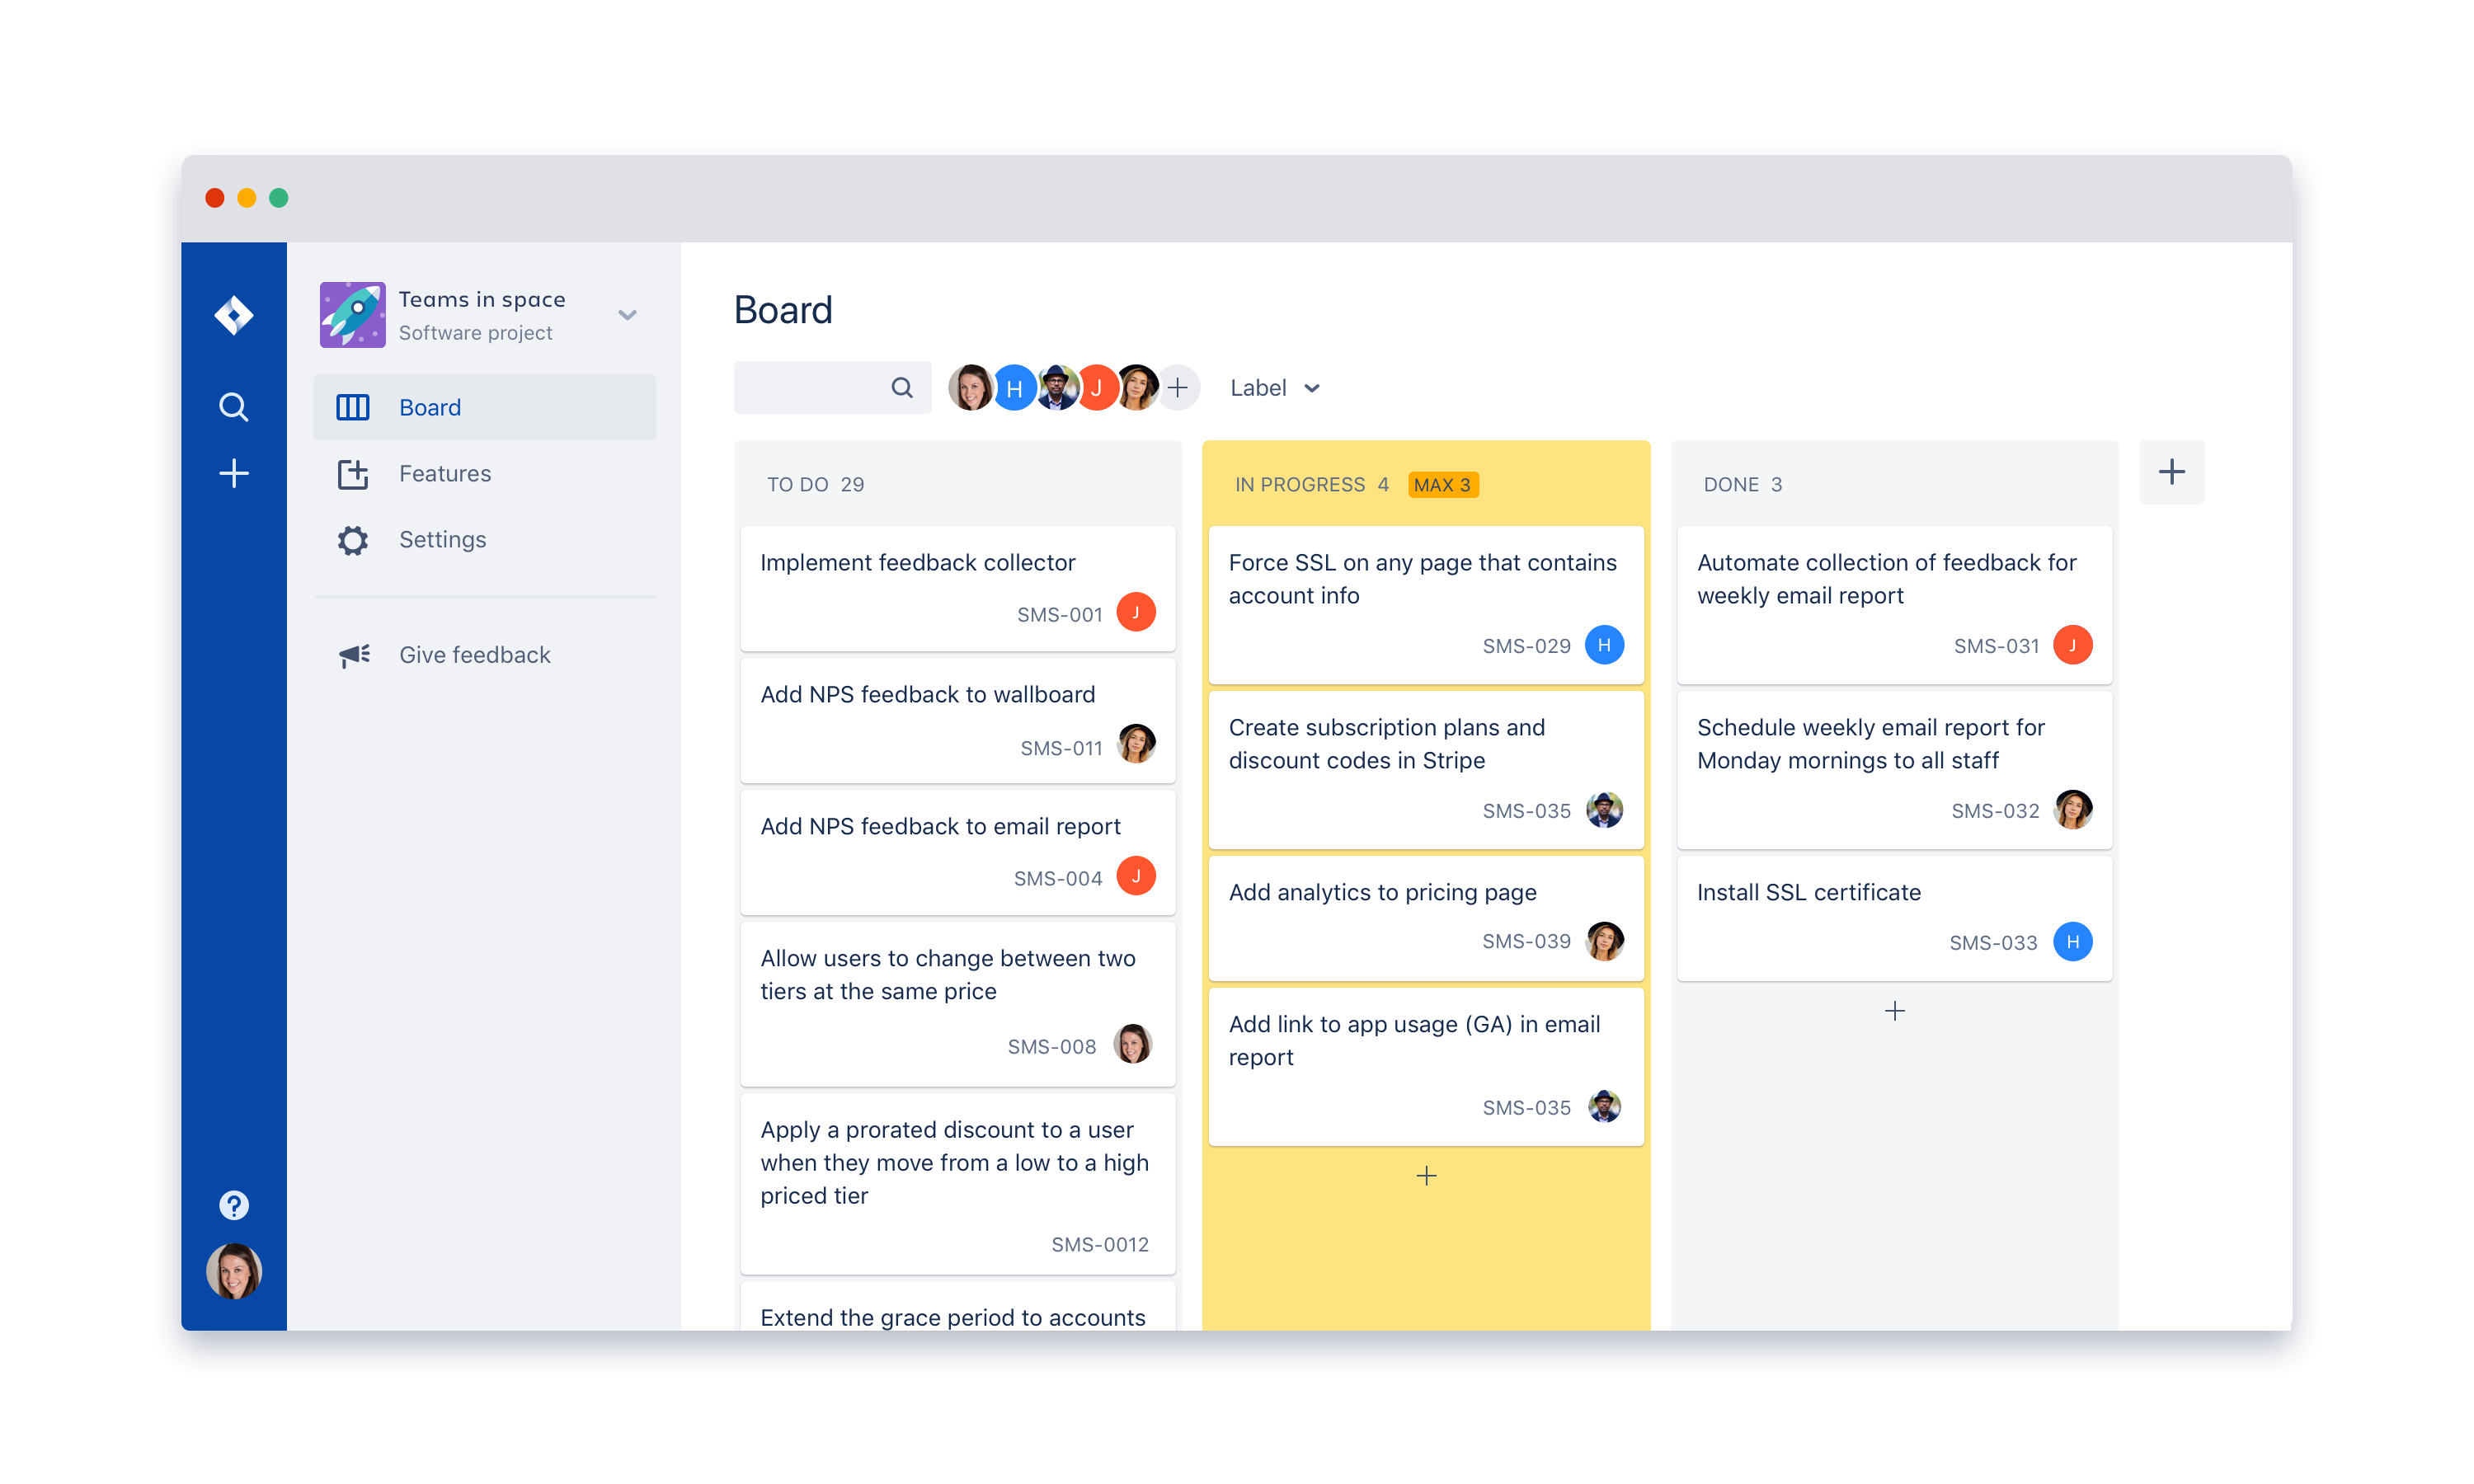
\includegraphics[width=1\textwidth]{Resources/kanban_board_example.png}
\caption{Beispiel eines Kandan-Boards}
\label{fig:kanban_board_example}
\end{figure}

Insgesamt bietet Kandan eine einfache und effektive Möglichkeit, den Fortschritt unseres Plotter-Projekts zu verwalten und sicherzustellen, dass wir kontinuierlich Verbesserungen vornehmen und auf unsere Ziele hinarbeiten.

\section{Dokumentation Anforderungsanalyse}

\section{Fazit}

\section{Arbeitstagebuch(Planung)}

\section{Arbeitstagebuch(Umsetzung)}

\section{Kundentests}


\end{document}
